\chapter{Kolmogorov Complexity vs. Shannon Entropy}
\label{ch:kolmogorov}

In the preceding chapters, we have heavily relied on Shannon entropy, $H(X)$, as the foundational measure of information. Shannon's formulation is inherently probabilistic: it quantifies the uncertainty, or average surprise, associated with a random variable $X$ drawn from a known probability distribution $P$. If we are transmitting messages over a noisy channel, Shannon entropy provides the fundamental lower bound on the expected number of bits required per symbol. However, this definition harbors a profound philosophical and practical limitation: it applies to an \textit{ensemble} of possible events, not to any individual object.

Consider a simple thought experiment. Suppose we observe two binary sequences of length $N = 1000$. The first sequence consists of alternating zeros and ones: \texttt{0101010101...}. The second sequence is generated by independent flips of a fair coin, resulting in something like \texttt{0110100111...}. If we view both sequences as particular realizations of a fair coin-flipping process, Shannon's theory assigns both sequences the exact same probability ($2^{-1000}$), and the source itself has an entropy of 1 bit per symbol. Thus, from the perspective of Shannon entropy, both sequences are equally ``surprising'' and contain the same amount of information. 

Yet, human intuition fiercely rebels against this equivalence. The first sequence is highly compressible. We can describe it succinctly in English as ``repeat '01' 500 times,'' or write a trivial computer program to generate it. The second sequence, lacking any discernible pattern, resists such compression; the shortest way to describe it is simply to list it entirely. Shannon's framework is fundamentally blind to this structural difference because it does not evaluate the internal regularities of individual sequences, only the probabilities of the ensembles from which they are drawn.

To capture the intrinsic information content of a specific, individual object, we must shift our perspective from probability to computation. This shift leads us to the domain of algorithmic information theory, pioneered independently by Andrey Kolmogorov, Ray Solomonoff, and Gregory Chaitin in the 1960s. The central concept of this theory is \textbf{Kolmogorov complexity}, denoted $K(x)$. Rather than asking ``How predictable is the random process that generated $x$?'', Kolmogorov complexity asks ``What is the length of the shortest computer program that can generate $x$ and then halt?''

Kolmogorov complexity provides a rigorous, universal measure of the absolute information content of an object. A sequence with discernible patterns will have a short generative program, and thus a low Kolmogorov complexity. A completely random sequence will have no program significantly shorter than the sequence itself, corresponding to a high Kolmogorov complexity. 

This chapter bridges the gap between these two profound pillars of information theory. We will formally define Kolmogorov complexity, establish its remarkable invariance properties, and prove the fundamental theorems that mathematically link the algorithmic complexity of individual strings to the Shannon entropy of random variables. By understanding how the deterministic structure of a single sequence connects to the statistical properties of ensembles, we lay the groundwork for understanding the Minimum Description Length (MDL) principle---a concept that will later prove crucial for demystifying generalization in deep neural networks.

\section{The Mathematical Core}

\begin{definition}[Universal Turing Machine]
A Turing machine $U$ is universal if it can simulate any other Turing machine. Specifically, there exists a prefix-free encoding such that for any Turing machine $T$ and input $x$, $U$ can take a program $p$ (which encodes $T$) and input $x$, and compute $T(x)$.
\end{definition}

\begin{definition}[Kolmogorov Complexity]
Let $U$ be a fixed universal Turing machine. The Kolmogorov complexity $K_U(x)$ of a binary string $x \in \{0,1\}^*$ with respect to $U$ is the length of the shortest binary program $p$ such that $U(p)$ outputs $x$ and halts:
\[ K_U(x) = \min_{p \in \{0,1\}^* : U(p) = x} \ell(p), \]
where $\ell(p)$ denotes the length of the program $p$ in bits. If no such program exists, $K_U(x) = \infty$.
\end{definition}

We usually restrict our attention to \textit{prefix-free} universal Turing machines (where no valid program is a prefix of another) to ensure that programs can be concatenated and decoded unambiguously. The complexity measure based on prefix-free machines is called prefix Kolmogorov complexity, often denoted simply as $K(x)$.

The immediate concern is that $K_U(x)$ seems inextricably tied to the arbitrary choice of the universal Turing machine $U$ (analogous to choosing a programming language like Python versus C). The Invariance Theorem resolves this anxiety.

\begin{theorem}[Invariance Theorem]
For any two universal Turing machines $U$ and $U'$, there exists a constant $c$, dependent only on $U$ and $U'$ but independent of $x$, such that for all strings $x \in \{0, 1\}^*$:
\[ K_{U'}(x) \le K_U(x) + c \]
\end{theorem}

\begin{proof}
Since $U'$ is a universal Turing machine, it can simulate $U$. There exists a compiler program $p_{U \to U'}$ of fixed length $\ell(p_{U \to U'}) = c$ that, when run on $U'$, reads an input program intended for $U$ and simulates its execution. Therefore, if $p$ is the shortest program for $x$ on $U$, the concatenated program $p_{U \to U'}p$ running on $U'$ will also output $x$. The length of this new program is $\ell(p) + c = K_U(x) + c$. Since $K_{U'}(x)$ is the length of the \textit{shortest} program on $U'$, we have $K_{U'}(x) \le K_U(x) + c$.
\end{proof}

Because of the Invariance Theorem, we typically drop the subscript and write $K(x)$, with the understanding that the measure is defined up to an additive constant $\mathcal{O}(1)$.

\begin{figure}[htpb]
    \centering
    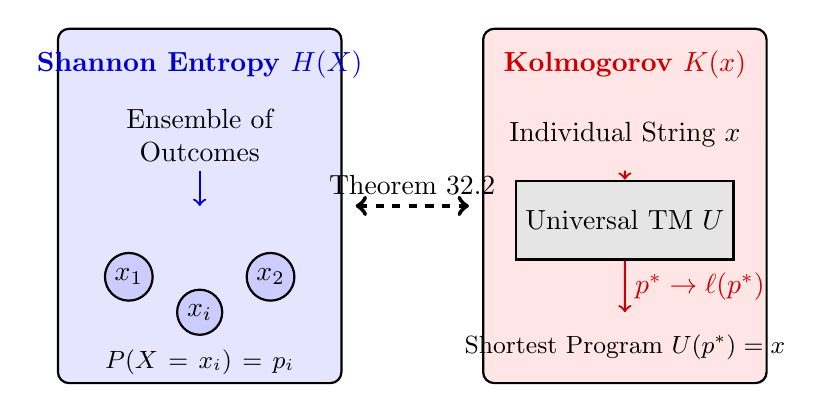
\begin{tikzpicture}[scale=0.9, thick]
        % Left diagram: Shannon Entropy
        \draw[fill=blue!10, rounded corners] (0, 0) rectangle (4, 5);
        \node[font=\bfseries, text=blue!80!black] at (2, 4.5) {Shannon Entropy $H(X)$};
        \node[text width=3.5cm, align=center] at (2, 3.5) {Ensemble of Outcomes};
        \draw[->, blue!80!black] (2, 3) -- (2, 2.5);
        \node[draw, circle, inner sep=2pt, fill=blue!20] (x1) at (1, 1.5) {$x_1$};
        \node[draw, circle, inner sep=2pt, fill=blue!20] (x2) at (3, 1.5) {$x_2$};
        \node[draw, circle, inner sep=2pt, fill=blue!20] (xi) at (2, 1) {$x_i$};
        \node[text width=3cm, align=center, font=\small] at (2, 0.3) {$P(X=x_i) = p_i$};
        
        % Right diagram: Kolmogorov Complexity
        \draw[fill=red!10, rounded corners] (6, 0) rectangle (10, 5);
        \node[font=\bfseries, text=red!80!black] at (8, 4.5) {Kolmogorov $K(x)$};
        \node[text width=3.5cm, align=center] at (8, 3.5) {Individual String $x$};
        \node[draw, rectangle, fill=gray!20, minimum width=2cm, minimum height=1cm] (tm) at (8, 2.3) {Universal TM $U$};
        \draw[->, red!80!black] (8, 3) -- (tm);
        \draw[->, red!80!black] (tm) -- (8, 1) node[midway, right] {$p^* \to \ell(p^*)$};
        \node[font=\small, align=center] at (8, 0.5) {Shortest Program $U(p^*) = x$};
        
        % Arrow between them
        \draw[<->, dashed, ultra thick] (4.2, 2.5) -- (5.8, 2.5) node[midway, above] {Theorem 32.2};
    \end{tikzpicture}
    \caption{Conceptual difference between Shannon Entropy, which evaluates the statistical uncertainty of an ensemble, and Kolmogorov Complexity, which evaluates the algorithmic information content of an individual string.}
    \label{fig:shannon_vs_kolmogorov}
\end{figure}

The relationship between the expected Kolmogorov complexity of strings drawn from a distribution and the Shannon entropy of that distribution is profound. We find that Shannon entropy serves as a lower bound for expected Kolmogorov complexity, and they are approximately equal up to the complexity of the distribution itself.

\begin{theorem}[Entropy and Expected Kolmogorov Complexity]
Let $X$ be a random variable taking values in a finite set $\mathcal{X} \subset \{0,1\}^*$ according to a computable probability distribution $P(x)$. Then, the expected Kolmogorov complexity of $X$ is bounded by the Shannon entropy $H(X)$:
\[ H(X) \le \mathbb{E}_{x \sim P}[K(x)] \le H(X) + K(P) + \mathcal{O}(1) \]
where $H(X) = - \sum_{x \in \mathcal{X}} P(x) \log_2 P(x)$ is the Shannon entropy in bits, and $K(P)$ is the length of the shortest program that computes the probability mass function $P(x)$.
\end{theorem}

\begin{proof}
\textbf{Lower Bound:} We rely on the fact that prefix-free programs form a uniquely decodable code. By Kraft's Inequality, for any prefix-free set of binary strings $S$, we have $\sum_{p \in S} 2^{-\ell(p)} \le 1$. 
Let $p^*_x$ be the shortest program generating $x$, so $\ell(p^*_x) = K(x)$. Since the Turing machine is prefix-free, the set of all such shortest programs is prefix-free. Thus, we can define a probability distribution $Q(x) = c \cdot 2^{-K(x)}$, where $c \ge 1$ is a normalization constant (since $\sum_x 2^{-K(x)} \le 1$). We know that the cross-entropy $H(P, Q) \ge H(X)$ due to the non-negativity of the Kullback-Leibler divergence $D_{\text{KL}}(P \parallel Q) \ge 0$.
\begin{align*}
    H(P, Q) &= -\sum_x P(x) \log_2 Q(x) \\
            &= -\sum_x P(x) \log_2 (c \cdot 2^{-K(x)}) \\
            &= -\sum_x P(x) (\log_2 c - K(x)) \\
            &= -\log_2 c + \sum_x P(x) K(x) \\
            &= -\log_2 c + \mathbb{E}_{x \sim P}[K(x)]
\end{align*}
Since $H(P, Q) \ge H(X)$ and $\log_2 c \ge 0$, we have:
\[ \mathbb{E}_{x \sim P}[K(x)] \ge H(P, Q) \ge H(X) \]

\textbf{Upper Bound:} We construct a specific decoding program to establish an upper bound on $K(x)$. According to Shannon's source coding theorem, there exists a prefix code (e.g., Huffman or Shannon-Fano code) that assigns a codeword $C(x)$ to each $x \in \mathcal{X}$ such that the expected codeword length is strictly less than $H(X) + 1$. To decode a specific string $x$, we can write a program that contains:
\begin{enumerate}
    \item The description of the distribution $P$ (length $K(P)$).
    \item The specific codeword $C(x)$ for the string $x$ (length $\ell(C(x)) \approx -\log_2 P(x)$).
    \item A constant-sized algorithmic routine that reads $P$, reconstructs the prefix tree, reads the codeword $C(x)$, decodes it, and halts (length $\mathcal{O}(1)$).
\end{enumerate}
The total length of this program is $K(P) + \ell(C(x)) + \mathcal{O}(1)$. Because $K(x)$ is the length of the \textit{shortest} program, it must be less than or equal to the length of this specific program:
\[ K(x) \le \ell(C(x)) + K(P) + \mathcal{O}(1) \]
Taking the expectation with respect to $P$:
\[ \mathbb{E}_{x \sim P}[K(x)] \le \mathbb{E}_{x \sim P}[\ell(C(x))] + K(P) + \mathcal{O}(1) \]
Since by Shannon's theorem $\mathbb{E}_{x \sim P}[\ell(C(x))] < H(X) + 1$, we can absorb the $+1$ into the constant term:
\[ \mathbb{E}_{x \sim P}[K(x)] \le H(X) + K(P) + \mathcal{O}(1) \]
This completes the proof.
\end{proof}

\begin{figure}[htpb]
    \centering
    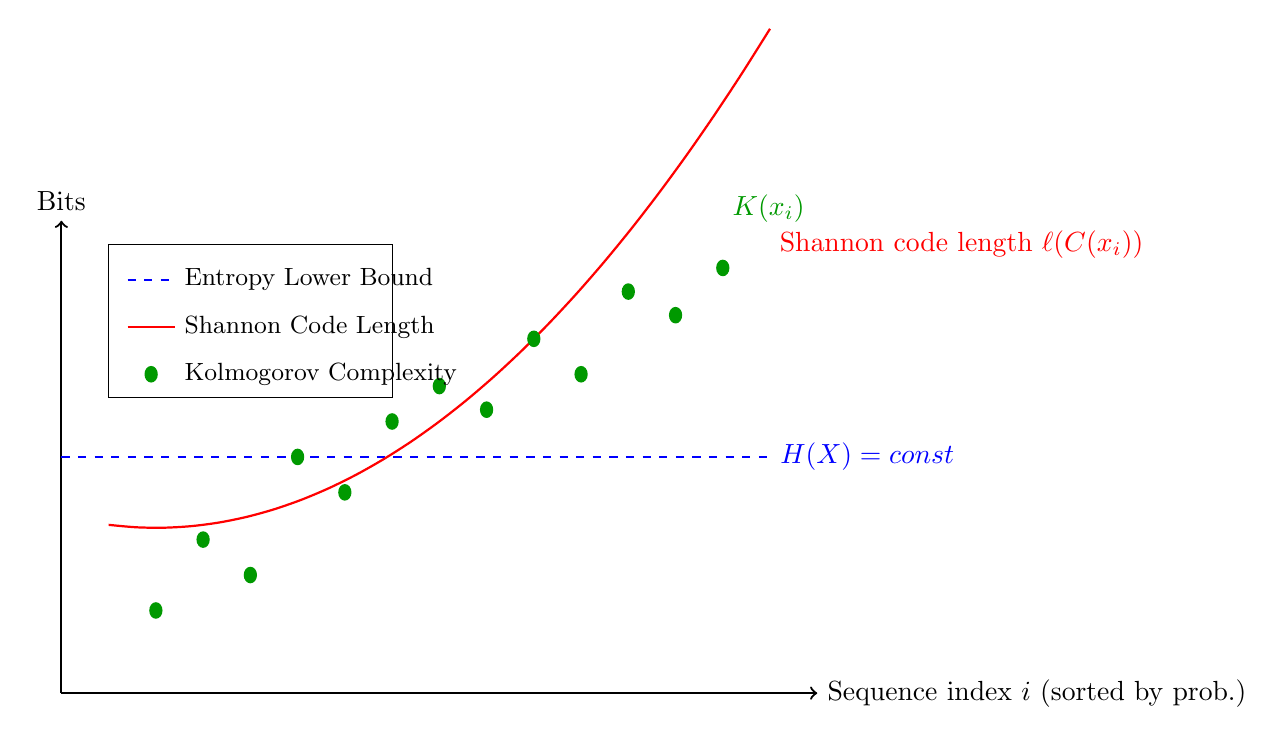
\begin{tikzpicture}[xscale=1.2, yscale=1.5]
        % Axes
        \draw[->, thick] (0, 0) -- (8, 0) node[right] {Sequence index $i$ (sorted by prob.)};
        \draw[->, thick] (0, 0) -- (0, 4) node[above] {Bits};
        
        % Shannon Entropy line
        \draw[blue, thick, dashed] (0, 2) -- (7.5, 2) node[right] {$H(X) = \text{const}$};
        
        % Shannon optimal code lengths
        \draw[domain=0.5:7.5, smooth, variable=\x, red, thick] plot ({\x}, {1.5 + 0.1*\x*\x - 0.2*\x});
        \node[red, right] at (7.5, 3.8) {Shannon code length $\ell(C(x_i))$};
        
        % Kolmogorov complexity dots
        \foreach \x/\y in {1/1.2, 1.5/1.8, 2/1.5, 2.5/2.5, 3/2.2, 3.5/2.8, 4/3.1, 4.5/2.9, 5/3.5, 5.5/3.2, 6/3.9, 6.5/3.7, 7/4.1} {
            \fill[green!60!black] (\x, \y - 0.5) circle (2pt);
        }
        \node[green!60!black, right] at (7, 4.1) {$K(x_i)$};

        % Legend box
        \draw[fill=white, draw=black] (0.5, 2.5) rectangle (3.5, 3.8);
        \draw[blue, thick, dashed] (0.7, 3.5) -- (1.2, 3.5);
        \node[right, font=\small] at (1.2, 3.5) {Entropy Lower Bound};
        \draw[red, thick] (0.7, 3.1) -- (1.2, 3.1);
        \node[right, font=\small] at (1.2, 3.1) {Shannon Code Length};
        \fill[green!60!black] (0.95, 2.7) circle (2pt);
        \node[right, font=\small] at (1.2, 2.7) {Kolmogorov Complexity};
    \end{tikzpicture}
    \caption{Visualizing the relationship between entropy, Shannon code lengths, and Kolmogorov complexity for individual sequences drawn from a non-uniform distribution. While $K(x_i)$ fluctuates for individual strings (as some strings are remarkably structured and simple to generate, deviating from their probabilistic code length), the expected value of $K(X)$ tightly tracks the Shannon entropy $H(X)$.}
    \label{fig:complexity_bounds}
\end{figure}

\subsection{Numerical Example}
Consider a biased coin that produces $1$ with probability $p=0.9$ and $0$ with probability $0.1$. The sequence length is $N = 1000$.
The Shannon entropy of the source is $N \cdot H(p) = 1000 \cdot (-0.9 \log_2 0.9 - 0.1 \log_2 0.1) \approx 469$ bits. 
If we draw a typical sequence $x$ from this distribution, we expect it to have roughly 900 ones and 100 zeros. By Theorem 32.2, the expected Kolmogorov complexity is roughly bounded by $469 + K(P) + \mathcal{O}(1)$. Describing a Bernoulli distribution requires only a few bits (to specify $p=0.9$), so $K(P)$ is vanishingly small relative to $N$. Thus, the shortest program to generate a \textit{typical} random sequence drawn from this biased distribution is about $469$ bits long. 

However, what if the sequence drawn happens to be exactly 1000 ones? The probability of this occurring is $0.9^{1000} \approx 1.7 \times 10^{-46}$, which is astronomically small, yet non-zero. The Shannon prefix code for this specific sequence would require approximately $-\log_2(0.9^{1000}) \approx 152$ bits. But the Kolmogorov complexity $K(\text{1000 ones})$ is incredibly small, perhaps just a few dozen bits: a trivial program that loops 1000 times suffices. This illustrates the core difference: Shannon code length is dictated solely by probability, whereas Kolmogorov complexity exploits deterministic structural simplicity.

\begin{horizon}
The relationship between algorithmic complexity and generalization in deep learning remains one of the most tantalizing theoretical frontiers. It is conjectured that the parameter matrices of neural networks that generalize well implicitly possess low Kolmogorov complexity. In this view, Stochastic Gradient Descent (SGD) does not merely seek any global minimum in the highly overparameterized loss landscape, but acts as a biased search algorithm that preferentially halts on functions with short algorithmic descriptions.

An open question is whether we can construct a rigorous, non-vacuous generalization bound for deep networks based purely on algorithmic information theory. Current PAC-Bayesian and Shannon-information bounds often suffer from the curse of dimensionality or become vacuous when the network can shatter the training data. If we can formally measure the complexity of the weight generation algorithm---or the length of the shortest program required to instantiate the network's function---future work might show that the true inductive bias of deep learning is perfectly synonymous with Solomonoff induction. 

To close this gap, one would need to translate the non-computable nature of Kolmogorov complexity into a tractable, empirical proxy (like Minimum Description Length), and prove that deep networks inherently minimize this proxy during gradient-based optimization on noisy data.
\end{horizon}

\section{Summary and Exercises}

\subsection*{Summary}
\begin{itemize}
    \item Shannon entropy $H(X)$ quantifies the statistical uncertainty of an ensemble, while Kolmogorov complexity $K(x)$ quantifies the algorithmic information of an individual object.
    \item The Invariance Theorem guarantees that Kolmogorov complexity is a universal measure, independent (up to a constant) of the underlying universal Turing machine.
    \item Theorem 32.2 proves that the expected Kolmogorov complexity of a random variable is tightly bounded by its Shannon entropy plus the complexity of the underlying probability distribution.
    \item While individual highly probable strings can have vastly different Kolmogorov complexities based on their internal structure, their average complexity aligns exactly with classical information theory.
\end{itemize}

\subsection*{Exercises}
\begin{enumerate}
    \item \textbf{Invariance Bounds.} Suppose $U_1$ is a Turing machine with an instruction set specialized for generating strings of alternating bits, while $U_2$ is a standard universal Turing machine. Describe a string $x$ where $K_{U_1}(x) \ll K_{U_2}(x)$ initially seems true. Explain how the Invariance Theorem still holds.
    \item \textbf{Complexity of Integers.} Let $x$ be the binary representation of an integer $N$. Show that $K(x) \le \log_2 N + \mathcal{O}(1)$.
    \item \textbf{Incomputability.} Prove that the Kolmogorov complexity function $K(x)$ is not computable. \textit{Hint: Use a proof by contradiction resembling the Berry paradox (``the smallest positive integer not definable in under sixty letters'').}
    \item \textbf{Conditional Complexity.} Define conditional Kolmogorov complexity $K(x|y)$ as the length of the shortest program that outputs $x$ given $y$ as input. Formulate an algorithmic analog to the chain rule of entropy $H(X, Y) = H(X) + H(Y|X)$. What extra terms might be necessary?
\end{enumerate}

% TODO-CITE: Ensure all named results are cited.
